\section{Vibração de Corpos Rígidos}

O som proveniente de objetos é geralmente principalmente por conta de sua vibração. Ao vibrar, o objeto movimenta o meio ao seu redor, criando ondas sonoras que serão propagadas. Podemos observar essa propriedade em instrumentos musicais: O prato de bateria, por exemplo, começa a vibrar ao ser atingido por uma baqueta, produzindo seu som característico. O corpo de um violão vibra quando suas cordas são tocadas, criando o som na frequência das cordas. Embora não consigamos observar a vibração a olho nu, é possível fazê-lo com câmeras especializadas (Ver \figref{fig:vibrating_cymbal}).

\begin{figure}[ht]
	\centering
	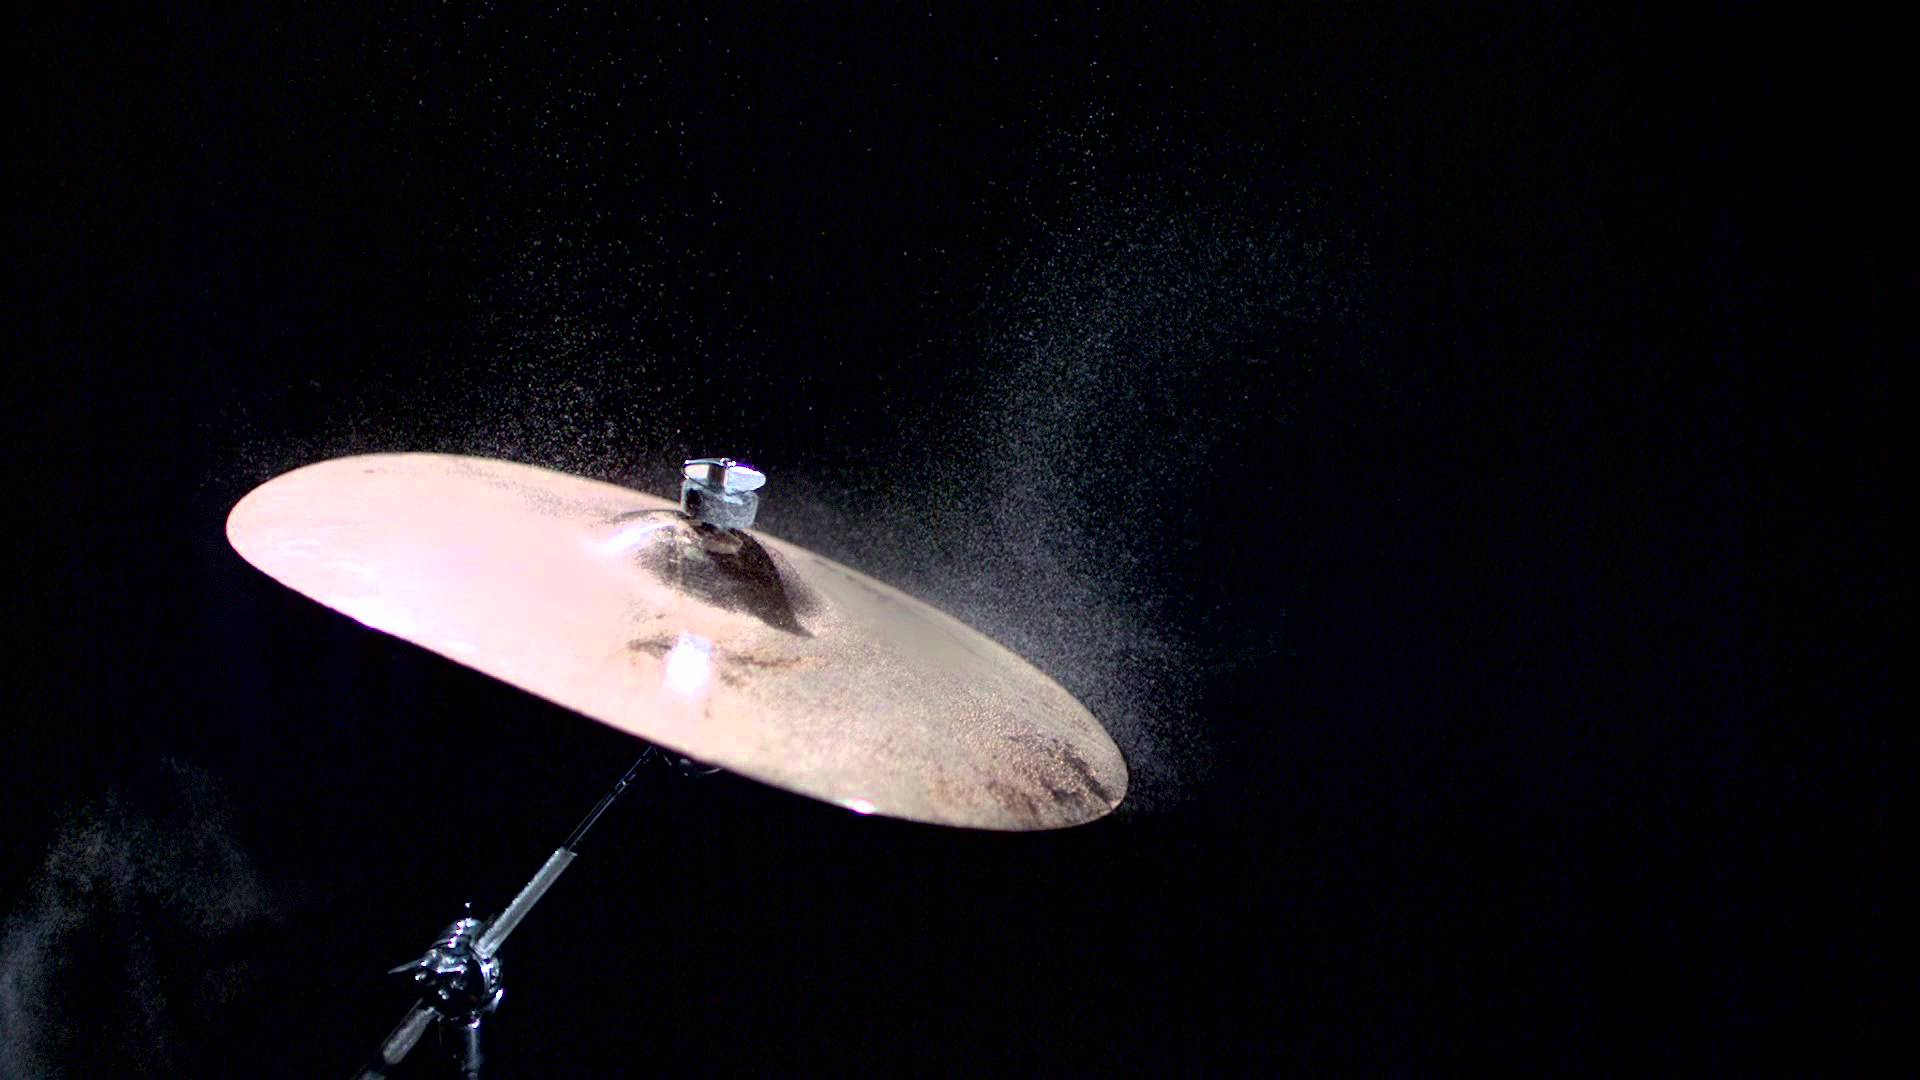
\includegraphics[width=0.7\textwidth]{mathematicalbackground/cymbal.jpg}
	\caption[Vibração de um prato de bateria.]{Vibração de um prato de bateria. O som produzido é gerado por conta dessa vibração\footnotemark}
	\label{fig:vibrating_cymbal}
\end{figure}

\footnotetext{Fonte: \url{https://i.ytimg.com/vi/kpoanOlb3-w/maxresdefault.jpg}. Acessado em 18 de Julho de 2016.}

Para entendermos melhor o comportamento da vibração de objetos, estudaremos o Modelo Elastodinâmico. 

\subsection{Modelo Elastodinâmico}
O modelo elastodinâmico \cite{shabana2012theory} é um dos modelos mais utilizados no estudo de vibrações. Esse modelo é amplamente utilizado em áreas como Engenharia Civil, Engenharia Mecânica, entre outras. 

O objeto de estudo do Modelo Elastodinâmico são os \emph{sistemas elastodinâmicos}. Um sistema elastodinâmico é um sistema composto por corpos $i$, cada um com massa $m_i$, e molas $(i,j)$, cada uma com constante elástica $k_{i,j}$. Um exemplo de sistema elastodinâmico é apresentado na \figref{1dbodysystem}.

\begin{figure}[ht]
	\centering
	\input{mathematicalbackground/1dbodysystem.tikz}
	\caption[Sistema elastodinâmico unidimensional]{Sistema elastodinâmico unidimensional. Cada nó tem massa $m_i$ e cada mola tem uma constante $k_{i,j}$}\label{1dbodysystem}
\end{figure}

De acordo com a Segunda Lei de Newton, sabemos que para cada corpo $i$,

\begin{equation}
f_{tot,i} = f_{int,i} + f_{ext, i} = m_i \cdot \ddot{p_i}
\label{2newton}
\end{equation}

onde $f_{ext,i}$ é a força externa,  $f_{int,i}$ a força interna, $m_i$ a massa do corpo e $\ddot{p_i}$ é a segunda derivada da posição (aceleração) do corpo $i$.  

Considere um sistema unidimensional com três corpos, como na \figref{1dbodysystem}, podemos escrever a Equação \eqref{2newton} na forma matricial:

\begin{equation}
	\begin{bmatrix}
		f_{tot,0}\\
		f_{tot_1}\\
		f_{tot_2}
	\end{bmatrix}
	=
	\begin{bmatrix}
		f_{int,0}\\
		f_{int,1}\\
		f_{int,2}
	\end{bmatrix}
	+\begin{bmatrix}
		f_{ext,0}\\
		f_{ext,1}\\
		f_{ext,2}
	\end{bmatrix}
	= 
	\begin{bmatrix}
		m_0 \cdot \ddot{p_0}\\
		m_1 \cdot \ddot{p_1}\\
		m_2 \cdot \ddot{p_2}
	\end{bmatrix}
	=
	\begin{pmatrix}
		m_0 & 0 & 0\\
		0 & m_1 & 0\\
		0 & 0 & m_2
	\end{pmatrix}
	\begin{bmatrix}
		\ddot{p_0}\\
		\ddot{p_1}\\
		\ddot{p_2}
	\end{bmatrix}
	= M\ddot{p}
\label{vecnewton}
\end{equation}

A matriz diagonal $M$ é chamada de \emph{Matriz de Massas} do sistema.

Seja $\vv{p_{eq}} = \begin{bmatrix}p_{eq,0} & p_{eq,1} & p_{eq,2}\end{bmatrix}^\intercal$ o vetor coluna que representa a posição de equilíbrio dos corpos na \figref{1dbodysystem}. Considere uma outra configuração $\vv{p}$. Se denotarmos por $\vv{u} = \vv{p}-\vv{p_{eq}}$ o vetor de deslocamento, podemos utilizar a Lei de Hooke para escrever:

\begin{eqnarray}
	\vv{f_{int}} =
	\begin{bmatrix}
		f_{int,0}\\
		f_{int,1}\\
		f_{int,2}
	\end{bmatrix}
	=&
	\begin{bmatrix}
		k_{0,1}(u_1 - u_0)&+& 0\\
		k_{0,1}(u_0 - u_1)&+& k_{1,2}(u_2 - u_1)\\
		0&+& k_{1,2}(u_1 - u_2)
	\end{bmatrix}\\
	=& 
	\begin{pmatrix}
		-k_{0,1} & k_{0,1} & 0\\
		k_{0,1} & -(k_{0,1}+k_{1,2}) & k_{1,2}\\
		0 & k_{1,2} & -k_{1,2}
	\end{pmatrix}
	\begin{bmatrix}
		u_0\\
		u_1\\
		u_2
	\end{bmatrix}\\
	=& Ku \label{stiffnessmatrix}
\end{eqnarray}

A matriz simétrica $K$ é chamada de \emph{Matriz de Rigidez} do sistema. Como $\vv{u} = \vv{p} - \vv{p_{eq}}$, temos que $\ddot{p} = \ddot{u}$. Desse modo, podemos substituir \eqref{stiffnessmatrix} em \eqref{vecnewton}:

\begin{equation}
	\vv{f_{ext}} + Ku = M\ddot{u}
\end{equation}

De modo semelhante, podemos utilizar essa equação para descrever sistemas com maior dimensionalidade. Um exemplo de tal sistema é apresentado na \figref{2dbodysystem}.

\begin{figure}[ht]
	\centering
	\input{mathematicalbackground/2dbodysystem.tikz}
	\caption[Sistema elastodinâmico bidimensional]{Sistema elastodinâmico bidimensional. Cada nó tem massa $m_i$ e cada mola tem uma constante $k_{i,j}$}\label{2dbodysystem}
\end{figure}

Para tal sistema, podemos descrever sua Matriz de Massas e sua Matriz de Rigidez. A Matriz de Massas $M$ é a matriz diagonal em blocos:

\begin{equation}
	M = \begin{pmatrix}
		M_0 & 0 & 0 & 0\\
		0 & M_1 & 0 & 0\\
		0 & 0 & M_2 & 0\\
		0 & 0 & 0 & M_3 
	\end{pmatrix}\\
	\text{onde }
	M_i = \begin{pmatrix}
		m_i & 0\\
		0 & m_i
	\end{pmatrix}
\end{equation}

A sua Matriz de Rigidez $K$ pode ser escrita como uma soma de matrizes $K_{i,j}$ para cada mola. Cada matriz $K_{i,j}$ tem uma simples estrutura em blocos\footnote{$M[l, c]$ representa o elemento da matriz $M$ presente na linha $l$ e coluna $c$}:

\begin{equation}
K_{i,j}[l, c] = \begin{cases}
	(l, c) = (i, i) \text{ ou } (l, c) = (j, j) \Rightarrow k_{i,j}R_{i,j} \\
	(l, c) = (i, j) \text{ ou } (l, c) = (j, i) \Rightarrow -k_{i,j}R_{i,j} \\
	\text{Caso contrário } \Rightarrow 0 \\
	\end{cases}\\
\end{equation}

$R_{i,j}$ é a matriz de rotação que alinha o vetor $\vv{p_j-p_i}$ com o eixo cartesiano $x$. A matriz $K_{1,3}$, por exemplo, teria a seguinte estrutura:

\begin{equation}
	K_{1,3} = \begin{pmatrix}
		0 & 0 & 0 & 0\\
		0 & k_{1,3}R_{1,3} & 0 & -k_{1,3}R_{1,3}\\
		0 & 0 & 0 & 0\\
		0 & -k_{1,3}R_{1,3} & 0 & k_{1,3}R_{1,3}
	\end{pmatrix}\\
\end{equation}

A generalização dessa equação é chamada de Equação da Elastodinâmica Linear: 

\begin{eqnarray}
M\ddot{u} + C\dot{u} + Ku &=& f_{ext} \in \mathbb{R}^n \label{elastodynamic} \\
&\text{onde}&\nonumber\\
u \in \mathbb{R}^{n} &\Rightarrow& \text{Vetor de deslocamento} \nonumber\\
f_{ext} \in \mathbb{R}^{n} &\Rightarrow& \text{Vetor de forças externas} \nonumber\\
M \in \mathbb{R}^{n\times n} &\Rightarrow& \text{Matriz de Massas} \nonumber\\
K \in \mathbb{R}^{n\times n} &\Rightarrow& \text{Matriz de Rigidez} \nonumber\\
C \in \mathbb{R}^{n\times n} &\Rightarrow& \text{Matriz de Amortecimento} \nonumber
\end{eqnarray}

Para objetos complexos, as matrizes são calculadas utilizando o Método dos Elementos Finitos \cite{hughes2012finite}. O método consiste em subdividir o objeto em pequenas partes, chamados de Elemento. As molas do sistema são utilizadas para unir os elementos que estão em contato. A massa dos Elementos e as constantes da mola são normalmente calculadas a partir das propriedades do material do objeto, como densidade ($\nicefrac{kg}{m^3}$), Módulo de Young ($Pa$) e Razão de Poisson \cite{shabana2012theory}. A Matriz de Amortecimento, no entanto, geralmente é calculada utilizando a aproximação de Rayleigh:
\begin{equation}
C = \alpha M + \beta{K}
\label{rayleighdamping}
\end{equation}

onde $\alpha$ e $\beta$ são constantes de dependem do material.

\subsection{Análise Modal}

Considere um sistema elastodinâmico. A sua Matriz de Massas $M$ é uma matriz diagonal positiva definida\footnote{Uma matriz $M \in \mathbb{R}^{n\times n}$ é dita positiva definida se, e somente se, $\forall v \in \mathbb{R}^n \Rightarrow v^\intercal M v > 0$. Uma definição equivalente é a de que todos os autovalores de $M$ são positivos.}. A sua matriz $K$ é a soma de matriz simétricas semi-positivas definidas, portanto ela também é uma matriz simétrica semi-positiva definida\footnote{Uma matriz $M \in \mathbb{R}^{n\times n}$ é dita semi-positiva definida se, e somente se, $\forall v \in \mathbb{R}^n \Rightarrow v^\intercal M v \ge 0$. Uma definição equivalente é a de que todos os autovalores de $M$ são não-negativos.}. Por tal razão, o problema dos autovalores generalizados está bem definido para estas matrizes \cite{parlett1980symmetric}. Isso significa é que possível encontrar uma base formada por vetores $v_i$, tais que:

\begin{equation}
	Kv_i = \lambda_i M v_i \label{eq:mode_scalar}
\end{equation}

Para cada par $(\lambda_i, v_i)$, o autovalor $\lambda_i = \omega_i^2$ está relacionado à frequência. De fato, dizemos que $\omega_i = 2\pi f_i$ é a \emph{Frequência Natural de Vibração}. Já o autovetor correspondente é o \emph{Modo Natural de Vibração}. É possível visualizar alguns modos de vibração na \figref{fig:sample_modes}.

\begin{figure}[ht]
\centering
\begin{subfigure}{0.32\textwidth}
	\centering
	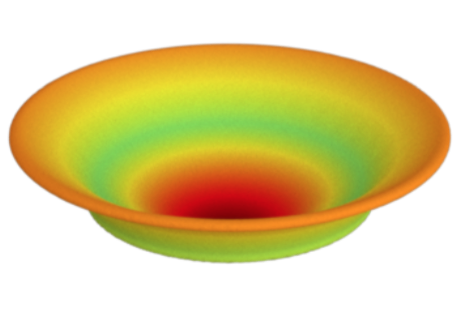
\includegraphics[height=0.15\textheight]{mathematicalbackground/modes/plate_4.png}
	\caption{Prato - Modo 4 - 2.6KHz}\label{fig:plates_4}
\end{subfigure}%
\begin{subfigure}{0.32\textwidth}
	\centering
	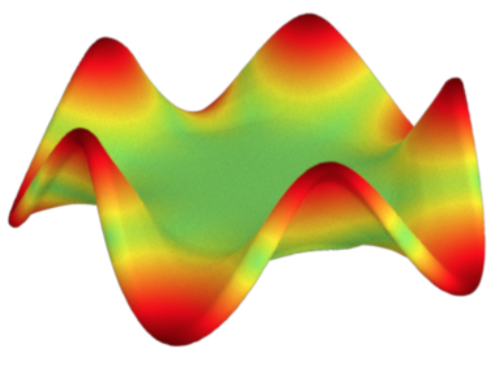
\includegraphics[height=0.15\textheight]{mathematicalbackground/modes/plate_9.png}
	\caption{Prato - Modo 9 - 4.9KHz}\label{fig:plates_9}
\end{subfigure}%
\begin{subfigure}{0.32\textwidth}
	\centering
	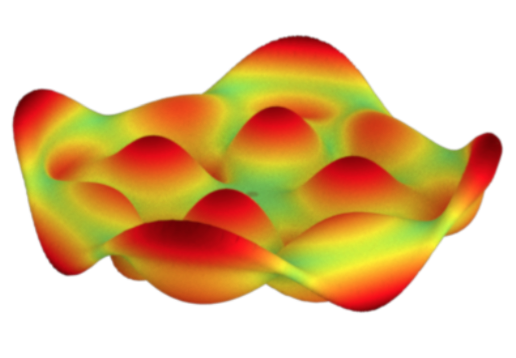
\includegraphics[height=0.15\textheight]{mathematicalbackground/modes/plate_48.png}
	\caption{Prato - Modo 48 - 16.6KHz}\label{fig:plates_48}
\end{subfigure}%

\begin{subfigure}{0.32\textwidth}
	\centering
	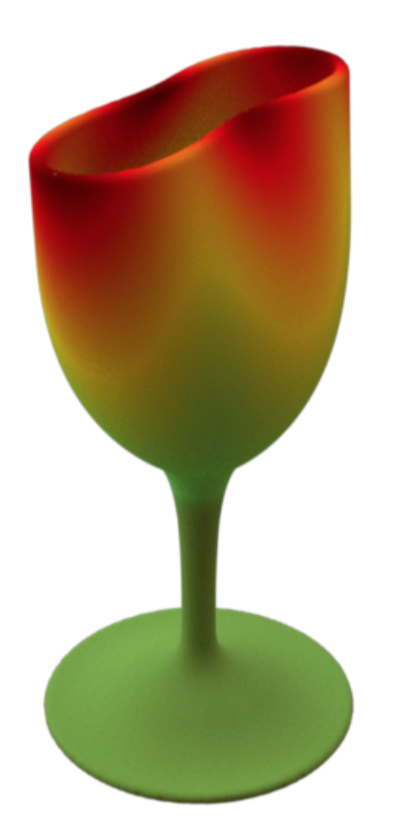
\includegraphics[height=0.2\textheight]{mathematicalbackground/modes/glass_3.png}
	\caption{Taça - Modo 3 - 1.9KHz}\label{fig:glass_3}
\end{subfigure}%
\begin{subfigure}{0.32\textwidth}
	\centering
	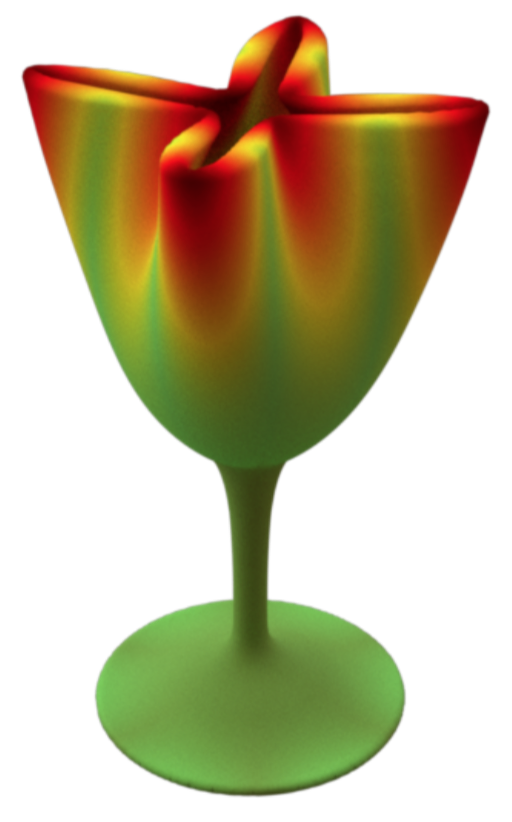
\includegraphics[height=0.2\textheight]{mathematicalbackground/modes/glass_15.png}
	\caption{Taça - Modo 15 - 9.3KHz}\label{fig:glass_15}
\end{subfigure}%
\begin{subfigure}{0.32\textwidth}
	\centering
	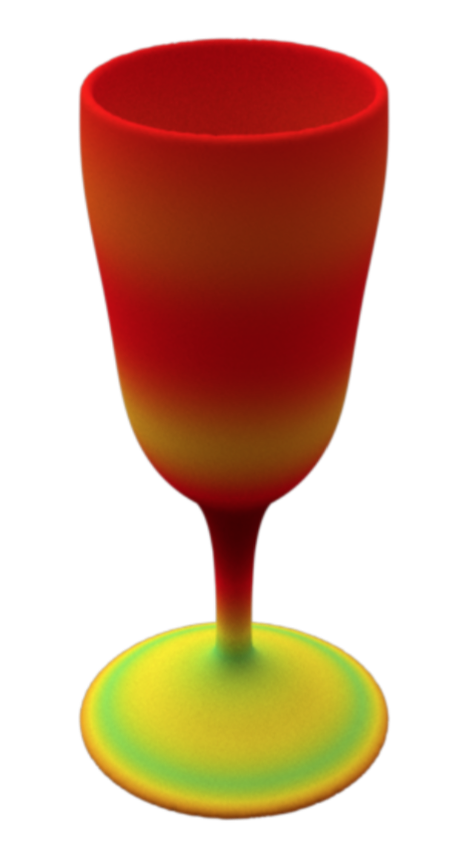
\includegraphics[height=0.2\textheight]{mathematicalbackground/modes/glass_33.png}
	\caption{Taça - Modo 33 - 16KHz}\label{fig:glass_33}
\end{subfigure}%
\caption[Modos de Vibração de objetos]{Modos de Vibração de objetos. Ao topo: Modos de vibração de um prato de cerâmica. Abaixo: Modos de vibração de uma taça de vidro. Fonte: \cite{langlois2014eigenmode}}
\label{fig:sample_modes}
\end{figure}

Podemos escrever a equação \eqref{eq:mode_scalar} também em sua forma matricial:

\begin{equation}
	KV = \Lambda M V
	\label{modematrix}
\end{equation}

$\Lambda$ é a matriz diagonal formada pelos autovalores $\lambda_i = \omega^2$ a $V$ é a matriz formada pelos vetores-coluna $v_i$. Em particular, pode-se escolher $V$ tal que ela seja ortogonal em relação à Matriz de Massas, isto é $V^\intercal M V = I$, onde $I$ é a matriz identidade. Nessa forma, dizemos que a matriz $\Lambda$ é a \emph{Matriz Espectral} do sistema e que $V$ é a \emph{Matriz Modal} do sistema.

Como $V$ representa uma base do espaço, então podemos encontrar um vetor $q$ tal que $u = Vq$. Se fizermos essa substituição na equação da elastodinâmica \eqref{elastodynamic} utilizando também a aproximação de Rayleigh \eqref{rayleighdamping} obteremos:

\begin{equation}
	MV\ddot{q} + (\alpha M + \beta{K})V\dot{q} + KVq = f_{ext}
\end{equation}

Podemos manipular a equação anterior:

\begin{eqnarray}
	f_{ext} =& MV\ddot{q} + (\alpha M + \beta{K})V\dot{q} + KVq \label{preexpansion}\\
	=& MV\ddot{q} + (\alpha MV + \beta KV)\dot{q} + KVq \label{afterexpansion}\\
	=& MV\ddot{q} + (\alpha MV + \beta \Lambda M V)\dot{q} + \Lambda M V \label{aftermodesubstition}\\
	\nonumber\\
	V^\intercal f_{ext} =& V^\intercal MV\ddot{q} + (\alpha V^\intercal MV + \beta V^\intercal \Lambda M V)\dot{q} + V^\intercal \Lambda M V\label{aftermultiplymode}\\
	=& \ddot{q} + (\alpha I + \beta\Lambda)\dot{q} + \Lambda q\label{finalmodeeqn}
\end{eqnarray}

Em \eqref{afterexpansion} expandimos o termo de $\dot{q}$. Em \eqref{aftermodesubstition}, aplicamos a igualdade \eqref{modematrix}. Em \eqref{aftermultiplymode}, multiplicamos ambos os lados da equação por $V^\intercal$ pela esquerda. Em \eqref{finalmodeeqn}, utilizamos o fato que $V$ é ortogonal em relação à $M$ e que a multiplicação por $\Lambda$ é comutativa (pois $\Lambda$ é diagonal).

Note que na equação final, todas as matrizes associadas aos termos $q$, $\dot{q}$ e $\ddot{q}$ são matrizes diagonais. Por tal razão, a equação diferencial multidimensional pode ser decomposta em várias equações diferenciais unidimensionais independentes:

\begin{equation}
	v_i^\intercal f_{ext} = \ddot{q_i} + (\alpha + \beta\omega_i^2)\dot{q_i} + \omega_i^2q_{i}
	\label{linear_modal_eqn}
\end{equation}

Se considerarmos o caso no qual uma força instantânea é aplicada no momento $t = 0$, isto é $v_i^\intercal f_ext(t) = \delta(t, 0)$ onde $\delta(x, y)$ é a função Delta de Dirac\footnote{A função Delta de Dirac é tal que $\delta(x, y) = 1$ se $x = y$ e $\delta(x, y) = 0$ caso contrário.} e que $q(0) = 0$, a solução da equação é da forma

\begin{equation}
	q(t) = k_1 e^{-k_2t} sin(k_3t)
\end{equation}

onde $k_1$, $k_2$ e $k_3$ são constantes (ver \figref{wave_mode}). Vale a pena salientar que a constante de frequência $k_3$ tem um valor próximo à frequência natural $\omega_i$. O seu valor é alterado de acordo com as constantes $\alpha$ e $\beta$.\footnote{Em especial, se $\alpha = \beta = 0$, temos que $k_3 = \omega_i$.}

\begin{figure}[ht]
	\centering
	\input{mathematicalbackground/wave_mode.tikz}
	\caption[Gráfico da solução da equação $\ddot{q}(t) + (\alpha + \beta\omega_i^2)\dot{q}(t) + \omega^2q(t) = f(t)$]{Gráfico da solução geral da equação $\ddot{q}(t) + (\alpha + \beta\omega_i^2)\dot{q}(t) + \omega^2q(t) = f(t)$ considerando $f(t) = \delta(t, 0)$. A frequência de $q(t)$ é próxima à frequência natural $\omega_i$.}\label{wave_mode}
\end{figure}

A possibilidade de decomposição em sistemas lineares independentes mostra que a vibração de um objeto pode ser expressa como a combinação linear de seus modos de vibração (ver \figref{plate_modes}). Veremos adiante como essa propriedade pode ser explorada para acelerar a simulação.

\begin{figure}[ht]
	\centering
	\input{mathematicalbackground/plate_modes.tikz}
	\caption[Composição de modos de vibração]{Composição de modos de vibração. A vibração de um objeto rígido pode ser expressa como combinação linear de diferentes modos de vibração regidos pela equação \eqref{linear_modal_eqn}}\label{plate_modes}
\end{figure}



